\subsection{SP1: reclutamiento por cuórum y cierre entero de coaliciones homogéneas}
\label{subsec:sp1}
\begingroup
\setlength{\parskip}{3pt plus 0.5pt}

SP1 sustituye demanda unitaria por cuotas $n_k\in\{1,2,3,4\}$. Con recursos suficientes, déficit y exceso caracterizan el cierre. Bajo escasez, el déficit lineal no distingue concentración de dispersión. QR cierra grupos y el cuórum favorece concentrarlos. Las poses solo fijan coste.

\subsubsection{Cuotas y escasez}

$\rho_D=(\sum_k n_k)/N$ distingue abundancia, ocupación crítica y escasez. La Figura~\ref{fig:sp1-scenario} muestra pertenencia lógica.

\begin{figure}[!htbp]
  \centering
  \begin{spdiagram}
    \spdrawarena{SP1 \textbar\ cuotas enteras y presión de demanda}
    \draw[sppanel] (0.35, 1.02) rectangle (4.35, 4.46);
    \draw[sppanel] (4.75, 1.02) rectangle (8.75, 4.46);
    \draw[sppanel] (9.15, 1.02) rectangle (13.15, 4.46);
    \node[spannotation] at (2.35, 4.18) {abundancia: $\rho_D<1$};
    \node[spannotation] at (6.75, 4.18) {crítico: $\rho_D=1$};
    \node[spannotation] at (11.15, 4.18) {escasez: $\rho_D>1$};

    \node[spload] (a1) at (1.45, 2.15) {$L_1$\\$n_1=1$};
    \node[spload] (a2) at (3.35, 2.15) {$L_2$\\$n_2=2$};
    \node[sprobot] (ar1) at (1.45, 3.22) {$R_1$};
    \node[sprobot] (ar2) at (2.85, 3.22) {$R_2$};
    \node[sprobot] (ar3) at (3.80, 3.22) {$R_3$};
    \node[sprobotfree,scale=0.80] (ar4) at (2.35, 1.35) {$R_4$};
    \draw[spassign] (ar1)--(a1); \draw[spassign] (ar2)--(a2); \draw[spassign] (ar3)--(a2);

    \node[spload] (c1) at (5.80, 2.15) {$L_1$\\$n_1=2$};
    \node[spload] (c2) at (7.70, 2.15) {$L_2$\\$n_2=2$};
    \node[sprobot] (cr1) at (5.35, 3.22) {$R_1$};
    \node[sprobot] (cr2) at (6.25, 3.22) {$R_2$};
    \node[sprobot] (cr3) at (7.25, 3.22) {$R_3$};
    \node[sprobot] (cr4) at (8.15, 3.22) {$R_4$};
    \draw[spassign] (cr1)--(c1); \draw[spassign] (cr2)--(c1);
    \draw[spassign] (cr3)--(c2); \draw[spassign] (cr4)--(c2);

    \node[spload] (s1) at (10.20, 2.15) {$L_1$\\$n_1=3$};
    \node[spload] (s2) at (12.10, 2.15) {$L_2$\\$n_2=2$};
    \node[sprobot] (sr1) at (9.65, 3.22) {$R_1$};
    \node[sprobot] (sr2) at (10.55, 3.22) {$R_2$};
    \node[sprobot] (sr3) at (11.45, 3.22) {$R_3$};
    \node[sprobot] (sr4) at (12.35, 3.22) {$R_4$};
    \draw[spassign] (sr1)--(s1); \draw[spassign] (sr2)--(s1);
    \draw[spcandidate] (sr3)--(s2); \draw[spcandidate] (sr4)--(s2);

    \draw[spassign] (0.30, 0.34)--(1.02, 0.34);
    \node[splegend,anchor=west] at (1.14, 0.34) {pertenencia cerrada};
    \draw[spcandidate] (4.15, 0.34)--(4.87, 0.34);
    \node[splegend,anchor=west] at (4.99, 0.34) {preferencia sin cierre};
    \node[sprobotfree,scale=0.42] at (8.65, 0.34) {};
    \node[splegend,anchor=west] at (8.91, 0.34) {robot inactivo};
  \end{spdiagram}
  \caption{SP1: cuotas cerradas con robots libres, uso total de flota y selección bajo escasez.}
  \label{fig:sp1-scenario}
  \viuownsource
\end{figure}

Sea $a_i\in\{0\}\cup\Loads$ la acción del robot $i$, con $0$ como inactividad. La ocupación y la coalición lógica son
\begin{equation}
 q_k(a)=\sum_{i\in\Robots}\mathbf1\{a_i=k\},\qquad
 C_k(a)=\{i\in\Robots:a_i=k\}.
 \label{eq:sp1-occupancy}
\end{equation}
Una carga cerrada cumple $q_k=|C_k|=n_k$. La cuota no expresa masa, fuerza, torque ni compatibilidad. SP2 introduce servicio y SP3 mecánica.

\subsubsection{Problema central de referencia y frontera de complejidad}

El oráculo dispone de la matriz global de costes normalizados $\kappa_{ik}\in[0, 1]$, de los valores adimensionales $v_k\geq0$ y de las cuotas $n_k$. Con $x_{ik},y_k\in\{0, 1\}$, resuelve
\begin{equation}
\label{eq:sp1-oracle}
\begin{aligned}
 \max_{x,y}\quad &\sum_{k\in\Loads}v_ky_k
 -\alpha\sum_{i\in\Robots}\sum_{k\in\Loads}\kappa_{ik}x_{ik}\\
 \text{sujeto a}\quad
 &\sum_{k\in\Loads}x_{ik}\leq1 &&(i\in\Robots),\\
 &\sum_{i\in\Robots}x_{ik}=n_ky_k &&(k\in\Loads),\\
 &x_{ik},y_k\in\{0, 1\}.&
\end{aligned}
\end{equation}
La igualdad excluye grupos parciales y exceso. $\alpha=0.15$ pondera coste y valor. Es un oráculo estático central.

La cuota no vuelve NP-difícil todo SP1. Con cargas obligatorias y $\rho_D\leq1$, expandir $n_k$ plazas produce asignación o flujo polinómico. Con cargas opcionales, $\sum_kn_ky_k\leq N$ y $\max\sum_kv_ky_k$ contiene mochila 0--1 (Anexo~\ref{app:sp1-complexity}). La dificultad está en seleccionar grupos completos bajo escasez.

\subsubsection{Métodos de comparación}

MILP-Q fija el techo global, mientras que Greedy-Q aporta una selección secuencial. Smith genera preferencias y QR grupos exactos, separando cuórum y cierre. Ambos usan ocupación global. En la Tabla~\ref{tab:sp1-methods}, $T_S$ son pasos Smith e $I_Q\leq K$ cierres.

\begin{table}[!htbp]
 \centering
  \caption{Comparación computacional de métodos en SP1.}
 \label{tab:sp1-methods}
  \viutablefont
  \setlength{\tabcolsep}{1.3pt}
  \renewcommand{\arraystretch}{0.92}
  \begin{tabularx}{\textwidth}{>{\raggedright\arraybackslash}p{2.2cm} >{\raggedright\arraybackslash}p{1.6cm} >{\raggedright\arraybackslash}p{2.35cm} >{\raggedright\arraybackslash}p{2.0cm} >{\raggedright\arraybackslash}p{1.75cm} Y}
  \toprule
  Método/fuente & Clase & Coste & Arq./información & Parámetros & Garantía/límite \\
  \midrule
  MILP-Q (reducción desde \textcite{karp1972reducibility}) & Obligatorio: P; selección opcional: NP-difícil & Optimizador exacto: exponencial en peor caso & Central; costes, cuotas y valores globales & $\alpha$, límite temporal/brecha & Óptimo solo con certificado; reducción en Anexo~\ref{app:sp1-complexity}. \\
  Greedy-Q (familia de recursos \parencite{zhangParker2013Resources}) & Selección opcional NP-difícil; heurística & $O(K^2N\log N)$ & Central; robots libres y todos los costes & $\alpha$, orden & Grupos enteros, sin cota y dependientes del orden. \\
  Smith continuo \parencite{sandholm2010population} & Relajación continua & $O(T_SN(K+1)^2)$ & Agregado exacto de ocupación; ejecución centralizada & $\Delta t,\allowbreak T_S,\allowbreak\epsilon,\allowbreak\beta,\allowbreak\lambda_O$ & Preferencias en el simplex. No cierra coaliciones ni hereda convergencia continua. \\
  Smith-QR & Cierre entero del problema NP-difícil & Smith $+\ {\scriptscriptstyle O(I_QKN\log N)}$;\allowbreak peor $O(K^2N\log N)$ & Preferencias, ordenación global y cuotas & Los anteriores, $\alpha$ & Ocupaciones $0$ o $n_k$. No es óptimo ni plenamente distribuido. \\
  Smith lineal + QR & Igual que Smith-QR & Igual que Smith-QR & Misma información; ablación del cuórum & $\beta=0$ & Conserva cierre; aísla la no linealidad de cuórum. \\
  Smith sin exceso & Relajación continua & $O(T_SN(K+1)^2)$ & Agregado exacto; sin penalización de exceso & $\lambda_O=0$ & Ablación sin garantía de cuota. \\
  \bottomrule
 \end{tabularx}
 \viusource{elaboración propia. Protocolo Smith basado en \textcite{sandholm2010population}}
\end{table}

CBBA es mono-ganador y no se ejecuta sin extensión verificada \parencite{choiBrunetHow2009CBBA}. \textcite{shehoryKraus1998Coalition,vigAdams2006Coalition} son contexto, no tratamientos.

\subsubsection{Juego de cardinalidad y mecanismo de cierre}

\begin{contribucion}{formulación de cuotas y caracterización de los equilibrios de SP1}
Para cargas obligatorias se generalizan el déficit y el exceso de SP0:
\begin{equation}
\begin{aligned}
 D_n(a)&=\sum_k\positivepart{n_k-q_k(a)}, &
 O_n(a)&=\sum_k\positivepart{q_k(a)-n_k},\\
 C(a)&=\sum_{i:a_i\neq0}\kappa_{i,a_i}, &
 J_Q(a)&=C(a)+\lambda_DD_n(a)+\lambda_OO_n(a),\\
 \Phi_Q(a)&=-J_Q(a), &
 U_i(a)&=\Phi_Q(a)-\Phi_Q(0,a_{-i}).
\end{aligned}
\label{eq:sp1-linear-game}
\end{equation}
Todos los términos son adimensionales. La utilidad es la contribución marginal: una desviación unilateral modifica $U_i$ exactamente como modifica $\Phi_Q$ \parencite{monderer1996potential}.

\begin{proposicion}[Cierre exacto bajo demanda realizable]
\label{thm:sp1-feasible-nash}
Si $\sum_kn_k\leq N$, $\kappa_{ik}\in[0,\kappa_{\max}]$ y $\lambda_D=\lambda_O=\lambda>\kappa_{\max}$, el juego de \eqref{eq:sp1-linear-game} es de potencial exacto y sus Nash puros son exactamente los perfiles con $q_k=n_k$ para toda carga. Toda secuencia de mejoras estrictas termina. Los máximos globales de $\Phi_Q$ son las asignaciones exactas de coste mínimo.
\end{proposicion}
\end{contribucion}
Un robot libre cubre déficit. Sin libres, la realizabilidad implica exceso y un traslado mejora. Toda desviación desde cuota exacta crea déficit o exceso por encima del ahorro espacial (Anexo~\ref{app:sp1-feasible-proof}).

La conclusión cambia bajo escasez.
\begin{contribucion}{límite formal del déficit lineal bajo escasez}
\begin{proposicion}[Degeneración del déficit lineal]
\label{thm:sp1-scarcity-degeneracy}
Si $N<\sum_kn_k$, todos los robots están activos y $q_k\leq n_k$ para toda carga, entonces
\[
 D_n(a)=\sum_kn_k-N,
\]
independientemente de la distribución de los robots. El potencial lineal no distingue por déficit entre completar una carga y dispersar los mismos robots entre grupos parciales.
\end{proposicion}
\end{contribucion}
La demostración completa está en el Anexo~\ref{app:sp1-scarcity-proof}.

El caso mínimo tiene dos cargas de cuota dos y dos robots: $(2,0)$ y $(1,1)$ presentan déficit dos, pero solo el primero completa una carga.
% El contraejemplo queda definido algebraicamente; su diagrama redundante se
\iffalse
\begin{figure}[!htbp]
 \centering
 \begin{spdiagram}
  \spdrawarena{SP1 \textbar\ contraejemplo de escasez: concentración frente a dispersión}
  \draw[sppanel] (0.35, 1.02) rectangle (6.35, 4.46);
  \draw[sppanel] (6.95, 1.02) rectangle (12.95, 4.46);

  \node[spannotation] at (3.35, 4.18) {concentración: $(q_1,q_2)=(2, 0)$};
  \node[spload] (cl1) at (2.05, 2.15) {$L_1$\\$n_1=2$};
  \node[spload] (cl2) at (5.00, 2.15) {$L_2$\\$n_2=2$};
  \node[sprobot] (cr1) at (1.35, 3.22) {$R_1$};
  \node[sprobot] (cr2) at (2.95, 3.22) {$R_2$};
  \draw[spassign] (cr1)--(cl1); \draw[spassign] (cr2)--(cl1);
  \node[spannotation] at (3.35, 1.30) {$D_n=2$; una carga completa};

  \node[spannotation] at (9.95, 4.18) {dispersión: $(q_1,q_2)=(1, 1)$};
  \node[spload] (dl1) at (8.55, 2.15) {$L_1$\\$n_1=2$};
  \node[spload] (dl2) at (11.55, 2.15) {$L_2$\\$n_2=2$};
  \node[sprobot] (dr1) at (7.80, 3.22) {$R_1$};
  \node[sprobot] (dr2) at (11.95, 3.22) {$R_2$};
  \draw[spcandidate] (dr1)--(dl1); \draw[spcandidate] (dr2)--(dl2);
  \node[spannotation] at (9.95, 1.30) {$D_n=2$; ninguna carga completa};

  \draw[spassign] (0.35, 0.34)--(1.05, 0.34);
  \node[splegend,anchor=west] at (1.18, 0.34) {asignación concentrada};
  \draw[spcandidate] (5.25, 0.34)--(5.95, 0.34);
  \node[splegend,anchor=west] at (6.08, 0.34) {asignación dispersa};
 \end{spdiagram}
 \caption{Contraejemplo de escasez: el déficit lineal es idéntico para concentración y dispersión, aunque el valor de servicio sea distinto.}
 \label{fig:sp1-scarcity-counterexample}
 \viuownsource
\end{figure}
\fi

\begin{contribucion}{formulación del incentivo de cuórum bajo escasez}
Para romper esa indiferencia se usa el beneficio exponencial normalizado y saturado
\begin{equation}
 \begin{aligned}
 B_{\beta,k}(q)&=
 \begin{cases}
 \dfrac{\exp\!\left(\beta\min\{q,n_k\}/n_k\right)-1}{\exp(\beta)-1},&\beta>0,\\[4pt]
 \dfrac{\min\{q,n_k\}}{n_k},&\beta=0,
 \end{cases}\\[4pt]
 \Phi_\beta(a)&=\sum_kv_kB_{\beta,k}(q_k)-\alpha C(a)-\lambda_OO_n(a).
 \end{aligned}
 \label{eq:sp1-quorum-benefit}
\end{equation}
Para $\beta>0$, los incrementos discretos antes de $n_k$ son crecientes y después del cuórum el beneficio se satura. En el contraejemplo con $n_1=n_2=2$, la concentración vale uno y la dispersión $2/(\exp(\beta/2)+1)<1$. Esto justifica el término, pero no prueba selección global para toda instancia.
\end{contribucion}
La derivación del incremento discreto y del contraejemplo se conserva en el Anexo~\ref{app:sp1-scarcity-proof}.

La relajación usa $\rho_{ik}\in[0,1]$ y $\widehat q_k=\sum_i\rho_{ik}$. La fitness combina incremento marginal, coste y exceso. Smith aplica Euler proyectado con $\Delta t=0.15$, 250 pasos y tolerancia $10^{-6}$. $\argmax_k\rho_{ik}$ no es una coalición ejecutable.

\begin{contribucion}{operador de cierre entero por ordenamiento y cuórum}
El operador $x=\mathcal Q_{\mathrm{QR}}(\rho)$ compara grupos completos entre los robots todavía libres, compromete el grupo de mayor puntuación positiva y repite hasta no poder cerrar otra cuota. Por construcción,
\begin{equation}
 \sum_kx_{ik}\leq1,\qquad \sum_ix_{ik}\in\{0,n_k\}.
 \label{eq:sp1-qr-invariants}
\end{equation}
QR agrega de forma determinista la matriz completa para aislar el efecto del cierre. Los resultados verifican \eqref{eq:sp1-qr-invariants}. La realización vecinal y su coste de consenso quedan fuera del alcance experimental de SP1.
\end{contribucion}

\subsubsection{Dinámica y cierre entero}

SP1 regula cardinalidad, aunque todavía no regula movimiento. Para una selección de cargas $y\in\{0, 1\}^K$, la salida estratégica por carga es
\begin{equation}
 z_{1,k}(a;y)=q_k(a)-n_ky_k,
 \qquad \boldsymbol z_1^{\mathrm{ref}}=\boldsymbol0.
 \label{eq:sp1-strategic-regulation}
\end{equation}
Con cargas obligatorias realizables, $y_k=1$ y $z_{1,k}=0$ indica cuota exacta. Bajo escasez, $y$ selecciona todo-o-nada y el objetivo es $q_k\in\{0,n_k\}$.

Cada robot realimenta su coste $\kappa_{ik}$, los parámetros públicos $(n_k,v_k)$ y una estimación $\widehat q_{ik}$ de la ocupación. La entrada estratégica es el flujo de preferencia entre acciones. Para fitness $f_{ik}$, el campo Smith utilizado antes del muestreo es
\begin{equation}
 \dot\rho_{ik}=
 \sum_{\ell}\rho_{i\ell}[f_{ik}-f_{i\ell}]_+
 -\rho_{ik}\sum_{\ell}[f_{i\ell}-f_{ik}]_+,
 \qquad
 \rho_i^{m+1}=P_{\Delta_i}\!\left(\rho_i^m+\Delta t\,\dot\rho_i^m\right).
 \label{eq:sp1-smith-feedback}
\end{equation}
QR convierte las preferencias en la acción discreta de~\eqref{eq:sp1-strategic-regulation}. Se usó $\widehat q_{ik}=q_k$ y la matriz completa. Ambos son datos globales y no un observador vecinal.

\begin{corolario}[Regulación exacta en el juego finito realizable]
\label{cor:sp1-strategic-regulation}
Bajo los supuestos de la Proposición~\ref{thm:sp1-feasible-nash}, una secuencia asíncrona de mejoras estrictas del juego finito alcanza en un número finito de revisiones $\boldsymbol z_1=\boldsymbol0$ para las cargas obligatorias.
\end{corolario}
La mejora finita se prueba en el Anexo~\ref{app:sp1-feasible-proof}. El resultado no se transfiere a Euler, Smith-QR ni escasez, sin estabilidad muestreada u optimalidad de $y$. Las poses siguen estáticas. SP2 cambia conteo por servicio, SP3 añade \emph{wrench} y SP4 movimiento.
\subsubsection{Diseño experimental}

El experimento usó 30 semillas por celda, $N\in\{8, 16\}$, seis presiones entre $0.50$ y $1.50$, cuotas homogéneas o mixtas 1--4 y geometría uniforme o agrupada: 1440 mundos pareados y 8640 ejecuciones. MILP-Q se resolvió con HiGHS. Se fijaron $\beta=2$, $\lambda_O=1.05$ y $\alpha=0.15$, y se barrió $\beta\in\{0, 0.5, 1, 2, 4, 8\}$. Las métricas fueron cierre, valor respecto al MILP, déficit, exceso, grupos parciales, brecha y CPU. Las comparaciones usaron Wilcoxon bilateral e intervalos bootstrap del 95\% con 2000 remuestras de mundos.

\subsubsection{Resultados}

\noindent\textbf{Verificación analítica.}
Doce enumeraciones reprodujeron la Proposición~\ref{thm:sp1-feasible-nash} y 14 controles verificaron contraejemplo y cuórum. Estas comprobaciones no prueban convergencia Smith muestreada.

\noindent\textbf{Cierre entero.}
En los 720 mundos de escasez, Smith continuo dejó en promedio el $10.95\%$ de la flota en grupos parciales y solo el $7.92\%$ de sus salidas cumplió el cierre lógico. Smith-QR produjo ocupaciones cero o exactas en todos los mundos. La diferencia Smith-QR menos Smith continuo en $R_{\mathrm{partial}}$ fue $-10.95$ puntos porcentuales (IC del 95\%: $[-12.07,-9.83]$, $p=5.59\times10^{-55}$). El efecto pertenece al operador QR: no demuestra que la preferencia continua converja a una asignación entera.

\noindent\textbf{Cuórum, calidad y resultado negativo.}
Con $\beta=2$, Smith-QR alcanzó el $95.17\%$ del valor del MILP en escasez. La diferencia pareada frente a Smith lineal + QR fue $+0.74$ puntos porcentuales (IC del 95\%: $[+0.21,+1.27]$, $p=0.0055$). Greedy-Q llegó al $98.71\%$ y superó a Smith-QR en $3.55$ puntos (IC del 95\%: $[2.99, 4.14]$, $p=3.00\times10^{-40}$). El contraste con la ablación de $\lambda_O$ tampoco mostró una reducción concluyente del exceso continuo: IC $[-2.27,+0.37]$ puntos y $p=0.390$. El cierre es necesario y el cuórum aporta una ventaja pequeña frente a su ablación, pero Smith-QR no supera al método voraz ni se confirma la hipótesis de exceso. Los seis tratamientos de la Tabla~\ref{tab:sp1-results} comparten los mismos mundos de escasez.

\begin{table}[!htbp]
 \centering
 \caption{Resultados en 720 mundos de escasez. CPU es una medida empírica, no una cota.}
 \label{tab:sp1-results}
 \scriptsize
 \setlength{\tabcolsep}{3.0pt}
 \renewcommand{\arraystretch}{1.05}
 \begin{tabular}{lrrrrrr}
\toprule
Método & $n$ & Cierre [\%] & Valor/MILP [\%] & Parciales [\%] & Exceso [\%] & CPU [ms] \\
\midrule
MILP-Q & 720 & 100.0 & 100.0 & 0.0 & 0.0 & 2.73 \\
Greedy-Q & 720 & 100.0 & 98.7 & 0.0 & 0.0 & 0.33 \\
Smith-QR & 720 & 100.0 & 95.2 & 0.0 & 0.0 & 63.00 \\
Smith lineal + QR & 720 & 100.0 & 94.4 & 0.0 & 0.0 & 59.40 \\
Smith continuo sin cierre ni exceso & 720 & 6.7 & 24.5 & 11.7 & 36.0 & 63.39 \\
Smith continuo (sin cierre) & 720 & 7.9 & 22.4 & 10.9 & 35.1 & 62.82 \\
\bottomrule
\end{tabular}

 \viuownsource
\end{table}

La preferencia continua y la asignación cerrada difieren: el cierre completa las cargas si $\rho_D\leq1$ y, bajo escasez, aparece la brecha de selección respecto al MILP (Figura~\ref{fig:sp1-regime-results}).
\begin{figure}[!htbp]
 \centering
 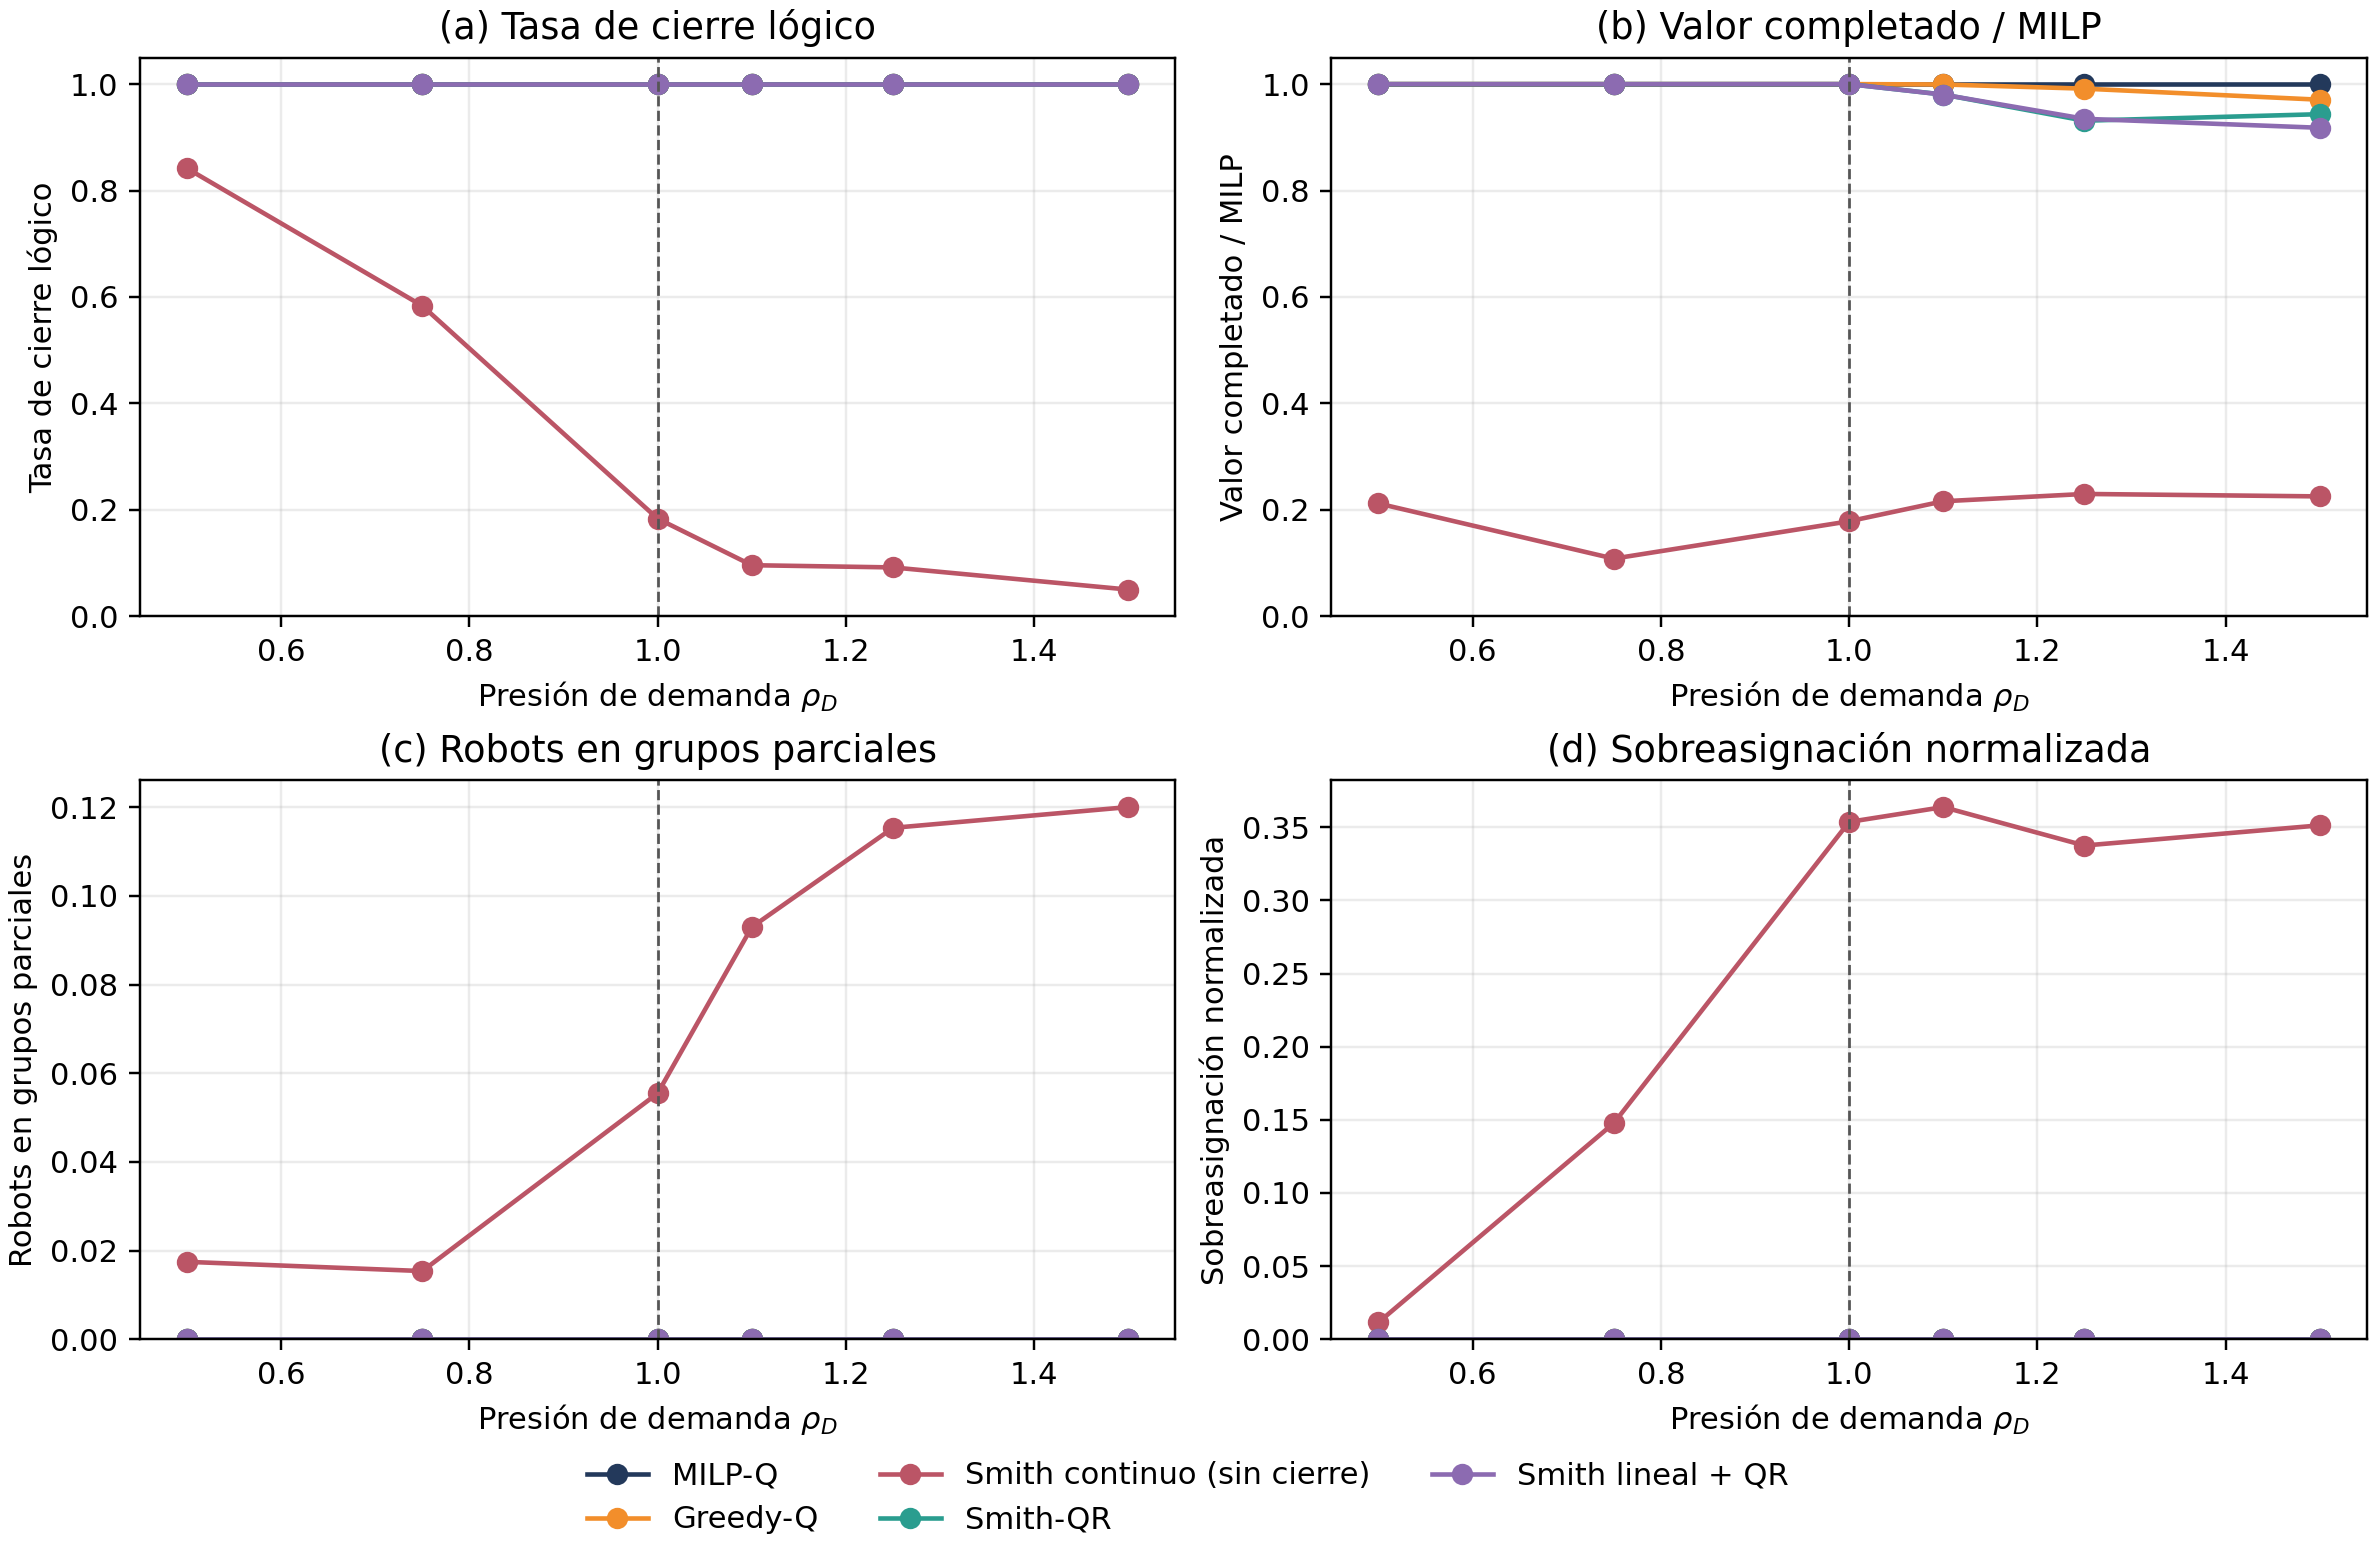
\includegraphics[width=0.65\textwidth]{../results/sp1/SP1_QUORUM_v1/figures/fig-sp1-regime-results.pdf}
 \caption{Resultados de desarrollo por presión de demanda, promediados sobre 240 mundos por nivel. La línea vertical separa realizabilidad y escasez.}
 \label{fig:sp1-regime-results}
 \viuownsource
\end{figure}

El mapa del Anexo~\ref{app:sp1-beta-map} muestra la sensibilidad a $\beta$. El valor $\beta=2$ no se interpreta como óptimo. Limitan la generalización la flota pequeña, el coste sintético, el cierre central y la ausencia de un comparador CBBA multi-ganador. La métrica de valor no incorpora transporte, seguridad ni mecánica.

\subsubsection{Síntesis}

En demanda realizable, los Nash puros cumplen las cuotas bajo la cota demostrada. Bajo escasez, QR elimina grupos parciales y, con ese cierre fijo, el cuórum mejora el valor en $0.74$ puntos porcentuales frente al beneficio lineal. Greedy-Q conserva mayor valor. SP2 sustituye la cuota por servicio operacional heterogéneo.
\endgroup
